% @HEADER
% ***********************************************************************
% 
%            Trilinos: An Object-Oriented Solver Framework
%                 Copyright (2001) Sandia Corporation
% 
% Under terms of Contract DE-AC04-94AL85000, there is a non-exclusive
% license for use of this work by or on behalf of the U.S. Government.
% 
% This library is free software; you can redistribute it and/or modify
% it under the terms of the GNU Lesser General Public License as
% published by the Free Software Foundation; either version 2.1 of the
% License, or (at your option) any later version.
%  
% This library is distributed in the hope that it will be useful, but
% WITHOUT ANY WARRANTY; without even the implied warranty of
% MERCHANTABILITY or FITNESS FOR A PARTICULAR PURPOSE.  See the GNU
% Lesser General Public License for more details.
%  
% You should have received a copy of the GNU Lesser General Public
% License along with this library; if not, write to the Free Software
% Foundation, Inc., 59 Temple Place, Suite 330, Boston, MA 02111-1307
% USA
% Questions? Contact Michael A. Heroux (maherou@sandia.gov) 
% 
% ***********************************************************************
% @HEADER

\documentclass[10pt,relax]{SANDreport}
\usepackage{amsmath,amsthm}
\usepackage{amssymb}
\usepackage{amsfonts}
\usepackage{palatino}

\def\choicebox#1#2{\noindent$\hphantom{th}$\parbox[t]{1.8in}{\sf
#1}\parbox[t]{4.5in}{#2}\\[0.8em]}

\author{Marzio Sala\\
Computational Mathematics and Algorithms Department \\
Sandia National Laboratories \\
P.O. Box 5800 \\
Albuquerque, NM 87185-1110
}

\title{Distributed Sparse Linear Algebra with PyTrilinos}
\SANDnum{SAND2005-XXXX}
\SANDauthor{Marzio Sala}

\SANDprintDate{June 2005}
\SANDreleaseType{Unlimited Release}

\newcommand{\PyTrilinos}{{PyTrilinos}}
\newcommand{\Trilinos}{{Trilinos}}
\newcommand{\TrilinosTM}{Trilinos \copyright}
\newcommand{\trilinos}{{Trilinos}}
\newcommand{\ifpack}{{IFPACK}}
\newcommand{\aztecoo}{{AztecOO}}
\newcommand{\amesos}{{Amesos}}
\newcommand{\epetra}{{Epetra}}
\newcommand{\ml}{{ML}}
\newcommand{\mb}[1]{{\mathbf {#1} }}
\newcommand{\teuchos}{{Teuchos}}
\newcommand{\triutils}{{Triutils}}
\newcommand{\metis}{{METIS}}
\newcommand{\note}[1]{\begin{center}\fbox{\bf #1}\end{center}}

\newcommand{\ie}{i.e., }
\newtheorem{assumption}{Assumption}[section]
\newtheorem{lemma}{Lemma}[section]
\newtheorem{proposition}{Proposition}[section]
\newtheorem{corollary}{Corollary}[section]
\newtheorem{theorem}{Theorem}[section]
\newtheorem{algorithm}{Algorithm}[section]
\newtheorem{definition}{Definition}[section]
\newtheorem{property}{Property}[section]
\newtheorem{interface}{Interface}[section]
\newtheorem{remark}{Remark}

\def\choicebox#1#2{\noindent$\hphantom{th}$\parbox[t]{3.0in}{\sf
#1}\parbox[t]{3.35in}{#2}\\[0.8em]}

\begin{document}

\maketitle

\begin{abstract}

\PyTrilinos\ is a collection of mathematical algorithms and utility functions
built on top of the Trilinos project~\cite{Trilinos-home-page}.  It adds
significant power to the interactive Python session by exposing the user to
high-level commands and classes for the creation, handling and usage of serial
dense and distributed sparse linear algebra objects. Using \PyTrilinos, an
interactive Python session becomes a powerful data-processing and
system-prototyping environment that can be used to test, validate, use and
extend serial and parallel numerical algorithms.
For some objects, \PyTrilinos\ implements
the popular Numeric module, gathering a variety of high-level distributed
sparse linear algebra functionalities together.

The main goal of this guide is to let you understand how to ``translate'' the
Trilinos constructs in PyTrilinos, and explain the most important differences.
The guide is {\sl not} a complete reference. If a set of options is available
for a given class of package, these options are not described here. The reader
still need to consult the manual of the underlying Trilinos package for a more
detailed insight.

\bigskip

\begin{center}

\includegraphics[height=4cm]{PyTrilinos.eps}
\end{center}

\end{abstract}

\SANDmain

\tableofcontents
\newpage

%-----------------------------------------------------------------------------
\section{Introduction}
\label{chap:introduction}
%-----------------------------------------------------------------------------

This document provides an overview of \PyTrilinos, version 2.x.  The 2.x
versions are completely revised and not compatible with earlier releases. The
major difference is a much wider coverage of Trilinos components and a better
integration with Python's lists and dictionaries, and support for MPI
programs. Some general Python facility is assumed such as could be acquired by
working through the tutorial in the Python
distribution~\cite{python-tutorial}.  It also is assumed that the reader is
somehow familiar with Trilinos, and knows how to install it.  It is of
paramount importance to remember that PyTrilinos is ``only'' a wrapper to
Trilinos, and therefore the reader cannot really understand PyTrilinos if he
or she is not somehow familiar with Trilinos.  We suggest
documents~\cite{Trilinos-tutorial, Trilinos-Users-Guide, Trilinos-home-page} 
to become familiar with the basic Trilinos
capabilities.

%-----------------------------------------------------------------------------
\subsection{Organization of this Document}
%-----------------------------------------------------------------------------

PyTrilinos reflects the Trilinos organization by presenting a series of {\sl
modules}, each of them wraps a given Trilinos package.  Algorithmic
capabilities are defined within independent Trilinos packages; a {\sl
package} is an integral unit usually developed by a small team of experts
in a particular area. 

The modules of \PyTrilinos\ covered in this document are:
\begin{itemize}
\item {\bf Epetra}. Epetra is a collection
of concrete classes that supports the construction and use of vectors, sparse
graphs, and dense and sparse matrices. It provides serial, parallel and
distributed memory capabilities. It uses the BLAS and LAPACK where possible,
  and as a result has good performance characteristics;
see~\cite{Epetra-Ref-Guide}.
%
\item {\bf EpetraExt}. This module offers input/output
capabilities, making it possible to read a matrix in Harwell/Boeing or
MatrixMarket format, or to read and write generic Epetra objects 
(like maps, matrices and vectors).
%
\item {\bf Triutils}. This module allows the creation of several matrices, 
  like the MATLAB's {\tt gallery} function, and it can be useful for examples
  and testing. 
%
\item {\bf Amesos}. This module contains a set of clear and consistent
interfaces to the following third-party serial and parallel sparse direct
solvers:
UMFPACK~\cite{umfpack-home-page},
PARDISO,
TAUCS,
SuperLU and SuperLU\_DIST~\cite{superlu-manual},
DSCPACK~\cite{dscpack-manual}, and 
MUMPS~\cite{mumps-manual}. See~\cite{Amesos-Reference-Guide} for more details. 
%
\item {\bf AztecOO}. This module contains preconditioned Krylov accelerators,
like CG, GMRES and several others, based on the popular Aztec library.
One-level domain decomposition preconditioners based on incomplete
factorizations are available.
%
\item {\bf IFPACK}. This module contains object-oriented algebraic
preconditioner
classes, compatible with Epetra and AztecOO.  It supports the construction and
the usage of parallel distributed memory preconditioners such as overlapping
Schwarz domain decomposition with several local solvers;
see~\cite{ifpack-guide} for more details.
%
\item {\bf ML}. This module contains a set of multilevel preconditioners based
on aggregation procedures for serial and vector problems. ML can take
advantage of the 
METIS~\cite{metis}
ParMETIS~\cite{parmetis} libraries to create the aggregates.
For a general introduction to ML and its applications, we refer to
the ML Users Guide~\cite{ml-guide}, and to the ML web site.
\end{itemize}

A description of the organization of  the linear algebra modules of
PyTrilinos, with some of the third-party libraries can be accessed,
is reported in Figure~\ref{fig:organization}.

\begin{figure}
\begin{center}
\includegraphics[width=12cm]{organization.eps}
\caption{Organization of the linear algebra modules of PyTrilinos.}
\label{fig:organization}
\end{center}
\end{figure}

%-----------------------------------------------------------------------------
\subsection{Suggested Configuration Options}
%-----------------------------------------------------------------------------

To fully take advantage of the presented modules of \PyTrilinos, Trilinos
should be compiled with the following options:
\begin{verbatim}
  --enable-teuchos    
  --enable-epetra     
  --enable-epetraext  
  --enable-amesos    
  --enable-ifpack     
  --enable-aztecoo     
  --enable-ml         
  --enable-triutils   
  --enable-python
\end{verbatim}

Users can decide to enable or disable any given module/package; however,
PyTrilinos without the Epetra module is almost an empty box.  As a matter of
fact, Epetra is the ``language'' of Trilinos, and offers a convenient set of
interfaces to define distributed linear algebra objects. Epetra supports
double-precision floating point data only (no single-precision or complex). 

\smallskip

After configuring and compiling Trilinos, one must install Trilinos 
(by typing \verb!make install!), in order to create PyTrilinos modules.
The installing procedure will copy all the Python modules in a subdirectory of
the directory specified with option \verb!--prefix=<inst-dir>!, for example \\
\verb!lib/python2.3/site-packages/PyTrilinos!. The reader might decide 
to add this directory to the \verb!PYTHONPATH! variable, for example using the 
bash shell command
\begin{verbatim}
% export PYTHONPATH=$PYTHONPATH:<inst-dir>/lib/python2.3/site-packages
\end{verbatim}

At this point, to use PyTrilinos  simply type
\begin{verbatim}
% python
Python 2.3 (#1, Sep 13 2003, 00:49:11) 
[GCC 3.3 20030304 (Apple Computer, Inc. build 1495)] on darwin
Type "help", "copyright", "credits" or "license" for more information.
>>> from PyTrilinos import <module-name>
\end{verbatim}
where \verb!<module-name>! is the name of the PyTrilinos module to be
imported, as later described.

If Trilinos was configured in parallel (MPI) mode, you cannot run PyTrilinos
interactively, and a Python script file must be created. This script can be
executed using an instruction of type
\begin{verbatim}
% mpirun -np 4 python ./my-script.py
\end{verbatim}

%-----------------------------------------------------------------------------
\subsection{Getting Information on \PyTrilinos}
%-----------------------------------------------------------------------------

PyTrilinos is under very active development, therefore small changes in usage
and calling sequences may occur. This
guide describes the ``stable'' features of PyTrilinos. For more up-to-date
details, the following sources of information can be consulted:
\begin{itemize}
\item {\bf General documentation}.
Please consult the web page \\
  \verb!http://software.sandia.gov/trilinos/packages/pytrilinos!
\item {\bf Mailing lists}. The reader can subscribe to the following lists:
\begin{verbatim}
pytrilinos-announce@software.sandia.gov
pytrilinos-users@software.sandia.gov
pytrilinos-developers@software.sandia.gov
\end{verbatim}
\item {\bf Sample code}. A variety of sample programs are available in the
\verb!<package-name>/python/example! subdirectory of several Trilinos
packages.
\item {\bf Bug report}.
Users and developers are encouraged to used Bugzilla to report
configuration problems, bugs, suggest enhancements, or require new features.
Bugzilla can be found on the web at\\
  \verb!http://software.sandia.gov/bugzilla!

If reporting a configuration problem or a bug, please attach the configure
script that has been used, and the compilation and/or run-time error.
\end{itemize}

%-----------------------------------------------------------------------------
\subsection{Notation Convention}
%-----------------------------------------------------------------------------

In this manuscript, typed commands are shown in this font:
\begin{verbatim}
% any_shell_command
>>> any_python_command
\end{verbatim}
The character \verb!%! indicates any shell prompt, while \verb!>>>! is the
Python prompt. Classes, function and module names are shown as \verb!Epetra!.
Mathematical entities are shown in italics.

%-----------------------------------------------------------------------------
\subsection{How to Reference This Document}
\label{sec:reference}
%-----------------------------------------------------------------------------

The PyTrilinos project can be referenced by using the following BiBTeX
citation information: 
\begin{verbatim}
@techreport{sparse05sala,
  title = "Distributed Sparse Linear Algebra With {P}y{T}rilinos",
  author = "Marzio Sala",
  institution = "Sandia National Laboratories",
  number = "SAND2005-XXXX",
  year = 2005
}
\end{verbatim}

%-----------------------------------------------------------------------------
\section{Serial Dense Linear Algebra}
\label{sec:serialdense}
%-----------------------------------------------------------------------------

Although PyTrilinos is focused on sparse, parallel linear algebra, some
capabilities are given to handle dense and serial linear algebra problems.
These capabilities are based on the Epetra wrapper for BLAS and LAPACK, and
therefore the serial dense module of PyTrilinos is computationally efficient.

We now report some basic operations involving serial dense objects. First, 
the {\tt Epetra} module must be imported, with the instruction
\begin{verbatim}
>>> from PyTrilinos import Epetra
\end{verbatim}
Serial dense matrices are defined by Epetra.SerialDenseMatrix objects; serial
dense vectors by Epetra.SerialDenseVector objects. As an example, 
we create the matrix $A$ and the vector $B$
\[
A = 
\begin{pmatrix}
1 & 3 & 5 \\
2 & 5 & 1 \\
2 & 3 & 8
\end{pmatrix}
, \quad \quad
B = 
\begin{pmatrix}
10 \\
  8 \\
  3
\end{pmatrix}
\]
with the following commands:
\begin{verbatim}
>>> A = Epetra.SerialDenseMatrix(3,3)
>>> X = Epetra.SerialDenseVector(3)
>>> B = Epetra.SerialDenseVector(3)
>>> A[0,0] = 1; A[0,1] = 3; A[0,2] = 5
>>> A[1,0] = 2; A[1,1] = 5; A[1,2] = 1
>>> A[2,0] = 2; A[2,1] = 3; A[2,2] = 8
>>> B[0] = 10;  B[1] = 8;   B[2] = 3
\end{verbatim}
We can  verify the result using 
\begin{verbatim}
>>> print A
Data access mode: Copy
A_Copied: yes
Rows(M): 3
Columns(N): 3
LDA: 3
1 3 5
2 5 1
2 3 8
>>> print B
Data access mode: Copy
A_Copied: yes
Length(M): 3
10 8 3 
\end{verbatim}
Matrix {\tt A} can be reshaped using \verb!A.Reshape(N, M)!; command
\verb!A.Shape(N, M)! reshapes and sets all the matrix elements to zero.  The
number of rows and columns of {\tt A} can be obtained using methods
\verb!A.N()! and \verb!A.M()!, respectively. \verb!A.NormOne()! and
\verb!A.NormInf()!  returns the 1- and $\infty-$norm of {\tt A}. The matrix
vector product is computed as \verb!A.Multiply(X, B)!;
\verb!SetUseTranspose()! toggles the use of $A$ or its transpose, $A^T$.
\verb!Scale(alpha)! scaled all the matrix elements by \verb!alpha!.

To solve the linear system
\begin{equation}
\label{eq:lin_sys}
A X = B,
\end{equation}
we first need to create an Epetra.SerialDenseSolver object, set the matrix and the vectors,
  then solve the linear system:
\begin{verbatim}
>>> Solver = Epetra.SerialDenseSolver()
>>> Solver.SetMatrix(A)
>>> Solver.SetVectors(X, B)
>>> Solver.Solve()
>>> print X
Data access mode: Copy
A_Copied: yes
Length(M): 3
-9.84 3.88 6.04 
\end{verbatim}
Alternatively, once can compute the inverse of $A$:
\begin{verbatim}
>>> Solver.Invert()
>>> print A

Data access mode: Copy
A_Copied: yes
Rows(M): 3
Columns(N): 3
LDA: 3
-1.48 0.56 0.16 
0.36 0.08 -0.12 
0.88 -0.36 0.04 
\end{verbatim}

%-----------------------------------------------------------------------------
\section{Building Sparse Linear Algebra Objects}
\label{sec:building}
%-----------------------------------------------------------------------------

%-----------------------------------------------------------------------------
\subsection{Communicators}
\label{sec:communicators}
%-----------------------------------------------------------------------------

Within PyTrilinos, all intra-processor communication are handled though the
communicator object Epetra.Comm, a pure virtual class. A concrete object can
simply be defined using a PyComm object:
\begin{verbatim}
>>> Comm = Epetra.PyComm()
\end{verbatim}
which returns an Epetra.SerialComm if PyTrilinos has been compiled in serial
mode, or an Epetra.MpiComm if PyTrilinos has support for MPI, using the
MPI\_COMM\_WORLD communicator. Start-up operations like a call to MPI\_Init()
  are performed by method Epetra.Init(). MPI is finalized by method
  Epetra.Finalize(). These two methods are empty functions for non-MPI runs,
  therefore we suggest to insert a call to Epetra.Init() as first instruction
  before the construction of the communicator, and to call Epetra.Finalize()
  as last Python instruction in all PyTrilinos scripts. Using this approach, 
PyTrilinos scripts are virtually identical for both serial and
parallel runs. A pictorial representation of how communication are handled in
the case of two  processors is given in Figure~\ref{fig:distributed}.

\begin{figure}
\begin{center}
\includegraphics[height=5cm]{distributed_object.eps}
\caption{All distributed PyTrilinos objects are based on the Epetra.MpiComm
  object, which takes care of calling MPI functions for intra-processor
    communications.}
\label{fig:distributed}
\end{center}
\end{figure}

%-----------------------------------------------------------------------------
\subsection{Maps}
\label{sec:maps}
%-----------------------------------------------------------------------------

Once a communicator has been defined as shown in
Section~\ref{sec:communicators}, the user has to specify the data layout for
any distributed linear algebra objects. In the Epetra lingo, this layout is
called a {\sl map}. PyTrilinos supports all maps allowed by Epetra. Here, we
report two examples, one for a simple linear map, and another for a more
realistic, non-structured map.

A linear maps containing 10
elements and with 0 as base index can be created as 
\begin{verbatim}
>>> Map = Epetra.Map(10, 0, Comm)
\end{verbatim}
The creation of a more realistic map is now reported. Let us suppose that the
map is composed by 9 elements, so that elements 0, 1, 5 and 6 are assigned to
processor 0, and elements 2, 3, 4, 7 and 8 to processor 1. We can create a
script file, here called {\tt exMap.py} as follows:
\begin{verbatim}
from PyTrilinos import  Epetra
Epetra.Init()
Comm = Epetra.PyComm()
if Comm.NumProc() != 2:
  raise Exception, "Must run w/ two processors"

if Comm.MyPID() == 0:
  MyGlobalElements = [0, 1, 5, 6];
else:
  MyGlobalElements = [2, 3, 4, 7, 8];
Map = Epetra.Map(-1, MyGlobalElements, 0, Comm);
print Map
Epetra.Finalize()
\end{verbatim}
By executing the program, we get:
\begin{verbatim}
[msala]> mpirun -np 2 python ./exMap.py
  Processor 0 of 2 total processor
  Processor 1 of 2 total processor

Number of Global Elements  = 9
Number of Global Points = 9
Maximum of all GIDs        = 8
Minimum of all GIDs        = 0
Index Base                 = 0
Constant Element Size      = 1

Number of Local Elements   = 4
Number of Local Points  = 4
Maximum of my GIDs         = 6
Minimum of my GIDs         = 0

         MyPID           Local Index        Global Index
             0                 0                 0
             0                 1                 1
             0                 2                 5
             0                 3                 6

Number of Local Elements   = 5
Number of Local Points  = 5
Maximum of my GIDs         = 8
Minimum of my GIDs         = 2

         MyPID           Local Index        Global Index
             1                 0                 2
             1                 1                 3
             1                 2                 4
             1                 3                 7
             1                 4                 8
\end{verbatim}

A list of elements assigned to the calling processor can be obtained by method
\verb!MyGlobalElements()!; for example, the instruction 
{\tt print Map.MyGlobalElements()} results in the output
\begin{verbatim}
[0, 1, 5, 6]
[2, 3, 4, 7, 8]
\end{verbatim}

%-----------------------------------------------------------------------------
\subsection{Basic Vector Operations}
\label{sec:vectors}
%-----------------------------------------------------------------------------

Once a map has been created as shown in Section~\ref{sec:maps}, then a
distributed vector can be created and used as follows:
\begin{verbatim}
>>> X = Epetra.Vector(Map)
>>> for i in range(0, X.MyLength()):
...   X[i] = i
... 
>>> print X
[ 0.  1.  2.  3.  4.  5.  6.  7.  8.  9.]
\end{verbatim}

Multi-vectors (that is, a collection of vectors all sharing the
same Map) can be created using typical Epetra
constructors. The following example creates a multivector {\tt X} which
contains 10 elements and 2 vectors, then sets the {\tt i-}th element of the
{\tt v-}vector, then print the result.
\begin{verbatim}
>>> for v in [0, 1]:
...   for i in range(0,X.MyLength()):
...     X[v,i] = 10 * v + i
...
>>> print X
     MyPID           GID               Value               Value  
         0             0                       0                  10
         0             1                       1                  11
         0             2                       2                  12
         0             3                       3                  13
         0             4                       4                  14
         0             5                       5                  15
         0             6                       6                  16
         0             7                       7                  17
         0             8                       8                  18
         0             9                       9                  19
\end{verbatim}
Several methods can be used to access and modify vectors and multivectors.
To set all the elements of a vector to a given value simply use {\tt
  X.PutScalar(0.0)}. To define random elements, use {\tt X.Random()}.

%-----------------------------------------------------------------------------
\subsection{Sparse Matrices}
\label{sec:matrices}
%-----------------------------------------------------------------------------

\epetra\ provides an extensive set of classes to create and fill
distributed sparse matrices. These classes allow row-by-row or
element-by-element constructions. Support is provided for common matrix
operations, including scaling, norm, matrix-vector multiplication and
matrix-multivector multiplication.
Using \epetra\ objects, applications do not need to know about the
particular storage format, and other implementation details such as data
layout, the number and location of ghost nodes. 

The process of creating a sparse matrix is more involved than the
process for dense matrices. This is because, in order to obtain
excellent numerical performance, one has to provide an estimation of
the nonzero elements on each row of the sparse matrix. (Recall that
dynamic allocation of new memory and copying the old storage into the
new one is an expensive operation.)

As an example, in this Section we will present how to construct a
distributed (sparse) matrix, arising from a finite-difference solution
of a one-dimensional Laplace problem. This matrix looks like
\begin{equation*}
A = \begin{pmatrix}
 2 & -1 &     &   &    \\
-1 &  2     & -1     &        &    \\
   & \ldots & \ldots & \ldots &  \\
   &        & -1     & 2      & -1 \\
   &        &        & -1     & 2
\end{pmatrix}.
\end{equation*}
First, we have to specify the number
of nonzeros per row. In general, this can be done in two ways:
\begin{enumerate}
\item Furnish an integer value, representing the number of nonzero
  element on each row (the same value for all the rows);
\item Furnish an integer vector \verb!NumNz!, of length
  \verb!NumMyElements()!, containing the nonzero elements of each row.
\end{enumerate}

We present here how to proceed using the first approach. The storage format is
inherited from the Epetra\_CrsMatrix class, which stores the matrix
row-by-row. 
\begin{verbatim}
>>> A = Epetra.CrsMatrix A(Epetra.Copy,Map,3);
\end{verbatim}
We can now create the matrix, by adding one row at-a-time.
To fill its values, we
need some additional variables: let us call them \verb!Indices! and
\verb!Values!. For each row, \verb!Indices! contains global column
indices, and \verb!Values! the correspondingly values.
\begin{verbatim}
>>> NumLocalRows = Map.NumMyElements()
>>> for ii in range(0, NumLocalRows):
...   i = Map.GID(ii)
...   if i == 0:
...     Indices = [i, i + 1]
...     Values  = [2.0, -1.0]
...   elif i == n - 1:
...     Indices = [i, i - 1]
...     Values  = [2.0, -1.0]
...   else:
...     Indices = [  i,  i - 1, i + 1]
...     Values  = [2.0,   -1.0,  -1.0]
...   Matrix.InsertGlobalValues(i, Values, Indices)
...
>>> ierr = Matrix.FillComplete()
\end{verbatim}
Method \verb!GID(ii)! returns the global ID of local row \verb!ii!.
Finally, we
transform the matrix representation into one based on local indices. The
transformation is required in order to perform efficient parallel
matrix-vector products and other matrix operations.
\begin{verbatim}
>>> A.FillComplete()
\end{verbatim}
This call to \verb!FillComplete()! will reorganize the internally stored
data so that each process knows the set of internal, border and external
elements for a matrix-vector product of the form $B = AX$. Also, the
communication pattern is established. As we have specified just one map,
\epetra\ considers that the the rows of $A$ are distributed among the
processes in the same way of the elements of $X$ and $B$.

To visualize the matrix, simply type
\begin{verbatim}
>>> print Matrix
\end{verbatim}

Another useful class is {\tt Epetra.FECrsMatrix}.
The most important additional feature provided by the
Epetra.FECrsMatrix with respect to Epetra.CrsMatrix, is the capability
to set non-local matrix elements. In the
example, we will set all the entries of a distributed matrix from
process 0. For the sake of simplicity, this matrix is diagonal, but more
complex cases can be handled as well.

\begin{verbatim}
>>> Matrix = Epetra.FECrsMatrix(Epetra.Copy, Map, 0)
>>> if Comm.MyPID() == 0:
...   for i in range(0, Map.NumGlobalElements()):
...     Indices = [i]
...     Values = [1.0]
...     Matrix.InsertGlobalValues(i, Indices, Values)
...
>>> Matrix.GlobalAssemble() 
>>> Matrix.FillComplete()
\end{verbatim}
Function \verb!SumIntoGlobalValues! adds the coefficients specified
in \verb!Indices! (as pair row-column) to the matrix, adding them to any
coefficient that may exist at the specified location. In a finite
element code, the user will probably insert more than one coefficient
at time (typically, all the matrix entries corresponding to an elemental
matrix). Method \verb!GlobalAssemble()! exchange data, so that 
each matrix element not owned by
process 0 could be sent to the owner, as specified by \verb!Map!. 

%-----------------------------------------------------------------------------
\subsection{Matrix Generation}
\label{sec:generation}
%-----------------------------------------------------------------------------

It is often convenient to generate matrices and linear systems corresponding
to well-known problems. Module Triutils makes it as simple as using the
MATLAB's {\tt gallery} function. For
details, we refer to the Trilinos tutorial~\cite[Chapter
5]{Trilinos-tutorial}. Here, we just show how to generate a matrix
corresponding to a 3D Laplacian on a structured Cartesian grid.  First, we
need to import modules \verb!Triutils! and \verb!Epetra!. Let {\tt nx, ny, nz}
be the number of nodes along the X-, Y- and Z-axis, respectively, and
\verb!Comm! an already created communicator.
  Then, we can simply write:
\begin{verbatim}
>>> nx = 100;
>>> ny = 100;
>>> nz = 100;
>>> Gallery = Triutils.CrsMatrixGallery("laplace_3d", Comm)
>>> Gallery.Set("nx", nx);
>>> Gallery.Set("ny", ny);
>>> Gallery.Set("nz", ny);
\end{verbatim}
The linear system matrix, solution and right-hand side are
obtained using
\begin{verbatim}
>>> Matrix = Gallery.GetMatrix();
>>> LHS = Gallery.GetStartingSolution();
>>> RHS = Gallery.GetRHS();
\end{verbatim}

These objects are automatically destroyed then the Gallery object is deleted.

%-----------------------------------------------------------------------------
\subsection{Input/Output}
\label{sec:io}
%-----------------------------------------------------------------------------

Module EpetraExt contains several utilities to read and write Epetra objects,
  in particular maps, vectors, and matrices. One of the goals of this module
  is to provide basic tools to facilitate exchange of data from codes based on
  Trilinos to codes based on PyTrilinos. For example, users may save on file
  the linear system produced by an application, then use an interactive Python
  session to optimize the parameters for its solution, or analyze the matrix
  (as explained in Section~\ref{sec:analyze}).

A {\tt Epetra.Map} object can be saved on file using the command
\begin{verbatim}
>>> FileName = "map.mm"
>>> EpetraExt.BlockMapToMatrixMarketFile(FileName, Map)
\end{verbatim}
or can be read from file as
\begin{verbatim}
>>> (ierr, Map2) = EpetraExt.MatrixMarketFileToBlockMap(FileName, Comm)
\end{verbatim}
where \verb!ierr! is the return error code. Analogously, 
\verb!Epetra.MultiVector!'s and \verb!Epetra.Crsmatrix!'s objects
can be saved on file as follows:
\begin{verbatim}
>>> EpetraExt.MultiVectorToMatrixMarketFile("x.mm", X)
>>> EpetraExt.RowMatrixToMatrixMarketFile("A.mm", A)
\end{verbatim}
then read as
\begin{verbatim}
(ierr, X2) = EpetraExt.MatrixMarketFileToMultiVector("x.mm", Map)
(ierr, A2) = EpetraExt.MatrixMarketFileToCrsMatrix("A.mm", Map)
\end{verbatim}

%-----------------------------------------------------------------------------
\section{Solving Distributed Sparse Linear Systems}
\label{sec:linear}
%-----------------------------------------------------------------------------

Let us consider again the solution of the linear system (\ref{eq:lin_sys}),
where $A \in \mathbb{R}^{n \times n}$ is a sparse linear operator, $X \in
\mathbb{R}^{n \times m}$ and $B \in \mathbb{R}^{n \times m}$ are the solution
and right-hand side, respectively. $n$ is the global dimension of the problem,
  and $m$ is the number of vectors in the multi-vectors $X$ and $B$. 
  (If $m = 1$, then $X$ and $B$ are ``normal'' vectors.)
Linear systems of type (\ref{eq:lin_sys}) arise in a variety of applications,
  and constitute the innermost computational kernel, and often the most
  time-consuming of several numerical algorithms. An efficient solver for
  Equation (\ref{eq:lin_sys}) is of fundamental importance for most PDE
  solvers, both linear and non-linear.

In \PyTrilinos, distributed sparse linear problems are represented by {\tt
  Epetra.LinearProblem} objects, which can be created either as
\begin{verbatim}
>>> Problem = Epetra.LinearProblem(Matrix, LHS, RHS)
\end{verbatim}
or as follows:
\begin{verbatim}
>>> Problem = Epetra.LinearProblem()
>>> Problem.SetOperator(Matrix)
>>> Problem.SetLHS(LHS)
>>> Problem.SetRHS(RHS)
\end{verbatim}
Methods \verb!GetMatrix()!, \verb!GetLHS()! and \verb!GetRHS()! can be used to
extract the linear system matrix, the solution vector, and the right-hand side
vector, respectively.

%-----------------------------------------------------------------------------
\subsection{Direct Solution of Sparse Linear Systems}
\label{sec:direct}
%-----------------------------------------------------------------------------

Probably, the most robust strategy to solve (\ref{eq:lin_sys}) is to factorize
the linear matrix $A$ into the product of two matrices $L$ and $U$, so that
$A = L \, U$, and 
the linear systems with $L$ and $U$ are readily solvable. Typically,
$L$ and $U$ are a lower and upper triangular matrix, respectively, and the
process is referred to as Gaussian elimination. 

Direct solution methods can be accessed through the Amesos module.
All Amesos objects are constructed from the function class
\verb!Amesos!.  Amesos allows a code to delay the
decision about which concrete class to use to implement the
Amesos.BaseSolver interface. The main goal of this class is to allow
the user to select any supported (and enabled at configuration time)
direct solver, simply changing an input parameter. Let us suppose that Amesos
has been configured and compiled with support for SuperLU. To solve the linear
system (\ref{eq:lin_sys}) with SuperLU, we first need to create a Solver
object,
\begin{verbatim}
>>> Factory = Amesos.Factory()
>>> Solver = Factory.Create("Superlu", Problem)
\end{verbatim}
Then, we can perform the symbolic and numeric factorizations using methods
\begin{verbatim}
>>> Solver.SymbolicFactorization()
>>> Solver.NumericFactorization()
\end{verbatim}
The numeric factorization phase will check whether a symbolic
factorization exists or not. If not, method
\verb!SymbolicFactorization()! is invoked.  Solution is computed (after
setting of LHS and RHS in the linear problem), using
\begin{verbatim}
>>> Solver.Solve()
\end{verbatim}
The solution phase will check whether a numeric factorization exists or
not. If not, method \\ \verb!NumericFactorization()! is called.
Users must provide the nonzero structure of the matrix for the symbolic
phase, and the actual nonzero values for the numeric
factorization. Right-hand side and solution vectors must be set before
the solution phase.
The object is deleted using
\begin{verbatim}
>>> del Solver
\end{verbatim}
  
Several parameters are available to toggle the selected Amesos solver.
To specify parameters, one can use Python's dictionaries:
\begin{verbatim}
>>> Factory = Amesos.Factory();
>>> Solver = Factory.Create(Type, Problem);
>>> AmesosList = {
...  "PrintTiming": ("bool", "true"),
...  "PrintStatus": ("bool", "true")
... }
...
>>> Solver.SetParameters(AmesosList);
\end{verbatim}
Please consult the Amesos manual~\cite{Amesos-Reference-Guide} for more
details.

%-----------------------------------------------------------------------------
\subsection{Preconditioned Krylov Accelerators}
\label{sec:iterative}
%-----------------------------------------------------------------------------

For sparse matrix, the major inconvenience of direct solution methods is that
the $L$ and $U$ factors are typically much denser than the original matrix
$A$, making Gaussian elimination too memory demanding for large scale
problems. Moreover, the factorization process is inherintly serial, and
parallel factorization algorithms can be successfully used only with a
relatively modest number of processors. The
forward and back triangular solves typically exhibit very poor parallel speedup.

A very well known solution to this problem is to adopt an iterative solution
process, like conjugate gradient (CG) or GMRES. The rationale behind
iterative methods is that they only require (at least in their simplest form)
matrix-vector and vector-vector products, and both operations scale well for
sparse matrices. 

To adopt an non-preconditioned iterative solver (for example, CG), with 1550
maximum iterations and a tolerance of $10^{-5}$ on the relative residual,
  PyTrilinos requires the following instructions:
\begin{verbatim}
>>> Solver = AztecOO.AztecOO(Matrix, LHS, RHS)
>>> Solver.SetAztecOption(AztecOO.AZ_solver, AztecOO.AZ_cg)
>>> Solver.SetAztecOption(AztecOO.AZ_precond, AztecOO.AZ_none)
>>> Solver.Iterate(1550, 1e-5)
\end{verbatim}
Other solvers can be used by replacing \verb!AZ_cg! with, for example,
  \verb!AZ_gmres!, \verb!AZ_bicgstab!, \verb!AZ_tfqmr!.

Unfortunately, the convergence of
iterative methods is determined by the spectral properties of the matrix
$A$---typically, its condition number $\kappa(A)$. For
real-life problems, $\kappa(A)$ is ``large'', meaning that the iterative
solution method will converge slowly. To solve this problem,
the original linear system is replaced by 
\[
A P P^{-1} X = B
\]
where $P$, called {\sl preconditioner}, is an operator whose inverse aim to
represent the inverse of $A$, though being much cheaper to compute.
$P$ is chosen so that $AP^{-1}$ is easier to solver than $A$ 
(that is, it is better conditioned). 

\smallskip

Often, algebraic preconditioners are adopted, that is, $P$ is constructed by
manipulating the entries of $A$. This gives rise to the so-called incomplete
factorization preconditioners (ILU) or algebraic multilevel methods. 

Because ILU preconditioners do not scale well on parallel computers, a common
practice is to perform {\em local} ILU factorizations.  In this situation,
each processor computes a factorization of a subset of matrix rows and
columns independently from all other processors.  This additional layer of
approximation leads to a block Jacobi type of preconditioner across
processors, where each block is solved using an ILU preconditioner.  The
difficulty with this type of preconditioner is that it tends to become less
robust and require more iterations as the number of processors used
increases.  This effect can be offset to some extent by allowing {\em
overlap}.  Overlap refers to having processors redundantly own certain
rows of the matrix for the ILU factorization.  Level-1 overlap is defined
so that a processor will include rows that are part of its original set.
In addition, if row $i$ is part of its original set and row $i$ of $A$ has
a nonzero entry in column $j$, then row $j$ will also be included in the
factorization on that processor.  Other levels of overlap are computed
recursively. 

What we have just described is an example of one-level overlapping domain
decomposition (DD) preconditioners.  The basic idea of DD methods consists in
dividing the computational domain into a set of subdomains, which may or may
not overlap. We will focus on overlapping DD methods only, because they can be
re-interpreted as algebraic manipulation of the assembled matrix, thus
allowing the construction of black-box preconditioners. Overlapping DD methods
are often referred to as overlapping Schwarz methods. DD preconditioners can
be written as
\begin{equation}
  \label{eq:prec_dd}
  P^{-1} = \sum_{i=1}^M R_i^T B_i^{-1} R_i,
\end{equation}
where $M$ represents the number of subdomains,
$R_i$ is a rectangular Boolean matrix that restricts
a global vector to the subspace defined by the interior of the $i$th
subdomain, and $B_i$ approximates the inverse of 
\begin{equation}
  \label{eq:aztecoo_tilde_a}
  A_i = R_i A R_i^T ,
\end{equation}
for example, being its ILU factorization.

In PyTrilinos two ways are available to define DD preconditioners:
\begin{itemize}
\item Using the {\tt AztecOO}'s preconditioners. The specification starts with
\begin{verbatim}
>>> Solver.SetAztecOption(AztecOO.AZ_precond, AztecOO.AZ_dom_decomp)
\end{verbatim}
Next, to adopt an incomplete factorization of $A_i$ with one level of overlap
among the subdomains,
\begin{verbatim}
>>> Solver.SetAztecOption(AztecOO.AZ_subdomain_solve, AztecOO.AZ_ilu)
>>> ver.SetAztecOption(AztecOO.AZ_overlap, 1)
>>> ver.SetAztecOption(AztecOO.AZ_graph_fill, 1)
\end{verbatim}

\item Using the {\tt IFPACK}'s preconditioners. This requires the {\tt IFPACK}
module.
\begin{verbatim}
>>> Factory = IFPACK.Factory();
>>> Prec = Factory.Create("ILU", Matrix);
>>> IFPACKList = {
...   "fact: level-of-fill": ("int", "5")
... }
... 
>>> Prec.SetParameters(IFPACKList);
>>> Prec.Initialize();
>>> Prec.Compute();
>>> Problem = Epetra.LinearProblem(Matrix, LHS, RHS);
>>> Solver = AztecOO.AztecOO(Problem);
>>> Solver.SetPrecOperator(Prec)
>>> Solver.SetAztecOption(AztecOO.AZ_solver, AztecOO.AZ_gmres);
\end{verbatim}
\end{itemize}

\bigskip

Another class of preconditioners is given by multilevel preconditioners.
For certain combinations of iterative methods and linear systems, the
error at each iteration projected onto the eigenfunctions has components
that decay at a rate proportional to the corresponding eigenvalue (or
frequency).  Multilevel methods exploit this property~\cite{Briggs}
by projecting the linear system onto a hierarchy of increasingly
coarsened ``meshes" so that each error component rapidly decays on at
least one coarse ``mesh."  The linear system on the coarsest ``mesh",
called the coarse grid problem, is solved exactly.  The iterative method
is called the smoother, as a reflection of its diminished role as a way
to damp out the high frequency error.  The grid transfer (or
interpolation) operators are called restriction and
prolongation operators.

Multilevel methods are characterized by the sequence of coarse spaces, the
definition of the operator each coarse space, the specification of the
smoother, and the restriction and prolongation operators.  Geometric multigrid
(GMG) methods  are multilevel methods that require the user to specify the
underlying grid, and in most cases a hierarchy of (not necessarily nested)
  coarsens grids.  Both the automatic generation of a grid-hierarchy for GMG
  and the specification of the ML, designed for unstructured problems, are
  beyond the scope of this document.

The development of algebraic multigrid (AMG)  (see \cite[Section 8]{Briggs}) 
has been motivated by the demand for multilevel methods that are
easier to use.  In AMG, both the matrix hierarchy and the prolongation
operators are constructed just from the stiffness matrix.  Recall that to use
Aztec00 or IFPACK,  a user must supply a linear system, a select a
preconditioning strategy.  In AMG, the only additional information required
from the user is to specify a coarsening strategy.

This Section requires to import the {\tt ML}, {\tt AztecOO} and {\tt Epetra}
modules. First, we set up the parameters for ML using a python dictionary:
\begin{verbatim}
>>> MLList = {
...  "max levels"        : ("int", "3"),
...  "output"            : ("int", "10"),
...  "smoother: type"    : ("string", "symmetric Gauss-Seidel"),
...  "aggregation: type" : ("string", "Uncoupled")
... };
\end{verbatim}
Then, we create the preconditioner and compute it,
\begin{verbatim}
>>> Prec = ML.MultiLevelPreconditioner(Matrix, False);
>>> Prec.SetParameterList(MLList);
>>> Prec.ComputePreconditioner();
\end{verbatim}
Finally, we set up the solver, and specifies to use \verb!Prec! as
preconditioner:
\begin{verbatim}
>>> Solver = AztecOO.AztecOO(Matrix, LHS, RHS)
>>> Solver.SetPrecOperator(Prec)
>>> Solver.SetAztecOption(AztecOO.AZ_solver, AztecOO.AZ_cg);
>>> Solver.SetAztecOption(AztecOO.AZ_output, 16);
>>> Solver.Iterate(1550, 1e-5)
\end{verbatim}

%-----------------------------------------------------------------------------
\section{Utilities}
\label{sec:utilities}
%-----------------------------------------------------------------------------

%-----------------------------------------------------------------------------
\subsection{Reading Harwell/Boeing Matrices}
\label{sec:hb}
%-----------------------------------------------------------------------------

The Triutils package makes it very easy to read a matrix stored in the popular
Harwell/Boeing format~\cite{hb}. The following lines read matrix {\tt
  fidap05}, which is freely available from the Matrix Market web site.
\begin{verbatim}
>>> from PyTrilinos import Triutils, Epetra
>>> Epetra.Init()
>>> Comm = Epetra.PyComm();
>>> Map, Matrix, LHS, RHS, Exact = Triutils.ReadHB("fidap05.rsa", Comm);
\end{verbatim}

%-----------------------------------------------------------------------------
\subsection{Matrix and Vectors Analysis}
\label{sec:analyze}
%-----------------------------------------------------------------------------

When working with linear systems, it is sometimes informative to be able to
obtain some basic statistical properties of the linear system matrix and
the corresponding vectors. 
The IFPACK package furnishes several utilities to accomplish this task.
Printed information concern the total number of rows and nonzeros, the average
number of nonzero elements per row, the band size, the number of (weakly)
  diagonally dominant rows, and the Frobenius norm of the matrix. These
  information are cheap to compute and sometimes useful to understand the
  structure of a given matrix.

For example, after having loaded matrix as reported in Section~\ref{sec:hb},
  we can analyze the structure of the matrix with the command
\begin{verbatim}
IFPACK.AnalyzeMatrix(Matrix)
\end{verbatim}
which results in the following output:
\begin{verbatim}
================================================================================
Label                          = Epetra::CrsMatrix
Global rows                    = 27
Global columns                 = 27
Stored nonzeros                = 279
Nonzeros / row                 = 10
Estimated storage (Mbytes)     = 0.003456

Actual nonzeros                = 279
Nonzeros in strict lower part  = 126
Nonzeros in strict upper part  = 126

Empty rows                     = 0                    ( 0 %)
Dirichlet rows                 = 0                    ( 0 %)
Diagonally dominant rows       = 0                    ( 0 %)
Weakly diag. dominant rows     = 0                    ( 0 %)

Maximum bandwidth              = 20

                                 one-norm       inf-norm       Frobenius
                                 ========       ========       =========

A                              = 7.11112e+06    7.11112e+06    9.08534e+06
A + A^T                        = 7.11112e+06    7.11112e+06    9.08534e+06
A - A^T                        = 0              0              0

                                 min            avg            max
                                 ===            ===            ===

 A(i,j)                        = -1.18519e+06   0.0167264      2.37038e+06
|A(i,j)|                       = 259259         345679         2.37038e+06

 A(k,k)                        = 296298         954735         2.37038e+06
|A(k,k)|                       = 296298         954735         2.37038e+06

 sum_j A(k,j)                  = 1.96297e+06    3.57202e+06    7.11112e+06
================================================================================
\end{verbatim}

Command \verb!IFPACK.AnalyzeMatrixElements(Matrix)! and
\verb!IFPACK.AnalyzeVectorElements(RHS)! will produce the output:
\begin{verbatim}
================================================================================
Label of matrix = Epetra::CrsMatrix

Elements in [-1.185186e+06, -8.296300e+05) =         20 ( =  7.17 %)
Elements in [-8.296300e+05, -4.740738e+05) =          0 ( =  0.00 %)
Elements in [-4.740738e+05, -1.185176e+05) =         88 ( = 31.54 %)
Elements in [-1.185176e+05, +2.370387e+05) =         96 ( = 34.41 %)
Elements in [+2.370387e+05, +5.925949e+05) =         60 ( = 21.51 %)
Elements in [+5.925949e+05, +9.481511e+05) =          0 ( =  0.00 %)
Elements in [+9.481511e+05, +1.303707e+06) =         10 ( =  3.58 %)
Elements in [+1.303707e+06, +1.659264e+06) =          0 ( =  0.00 %)
Elements in [+1.659264e+06, +2.014820e+06) =          0 ( =  0.00 %)
Elements in [+2.014820e+06, +2.370376e+06) =          4 ( =  1.43 %)
================================================================================
\end{verbatim}

\begin{verbatim}
================================================================================
Vector label = Epetra::Vector

Elements in [+0.000000e+00, +2.666667e-03) =         18 ( = 66.67 %)
Elements in [+2.666667e-03, +5.333333e-03) =          0 ( =  0.00 %)
Elements in [+5.333333e-03, +8.000000e-03) =          0 ( =  0.00 %)
Elements in [+8.000000e-03, +1.066667e-02) =          0 ( =  0.00 %)
Elements in [+1.066667e-02, +1.333333e-02) =          1 ( =  3.70 %)
Elements in [+1.333333e-02, +1.600000e-02) =          3 ( = 11.11 %)
Elements in [+1.600000e-02, +1.866667e-02) =          0 ( =  0.00 %)
Elements in [+1.866667e-02, +2.133333e-02) =          0 ( =  0.00 %)
Elements in [+2.133333e-02, +2.400000e-02) =          0 ( =  0.00 %)
Elements in [+2.400000e-02, +2.666667e-02) =          4 ( = 14.81 %)
================================================================================
\end{verbatim}

Finally, it is possible to print on file the sparsity pattern of the matrix
(here reported in Figure~\ref{fig:sparsity}) using the instruction
\begin{verbatim}
IFPACK.PrintSparsity(Matrix, "matrix.ps")
\end{verbatim}

\begin{figure}
\begin{center}
\includegraphics[height=5cm]{sparsity.ps}
\caption{Sparsity pattern of matrix {\tt fidap05} obtained using {\tt
  IFPACK.PrintSparsity()}.}
\label{fig:sparsity}
\end{center}
\end{figure}

%-----------------------------------------------------------------------------
\subsection{Timing}
%-----------------------------------------------------------------------------

Class {\tt Epetra.Time} can be used to track the elapsed CPU time as follows:
\begin{verbatim}
>>> Comm = Epetra.PyComm()
>>> Time = Epetra.Time(Comm)
>>> Time.ResetStartTime()
    ... do something here ...
>>> print "Elapsed time is ", Time.ElapsedTime()
\end{verbatim}

%-----------------------------------------------------------------------------
\subsection{Matrix-Matrix Operations}
%-----------------------------------------------------------------------------

The {\tt EpetraExt} module offers matrix-matrix operations. To add two matrices
(with compatible maps), do
\begin{verbatim}
EpetraExt.Add(A, False, 1.0, B, -1.0)
\end{verbatim}

%-----------------------------------------------------------------------------%
\bibliographystyle{plain}
\bibliography{guide}
%-----------------------------------------------------------------------------%
\end{document}


Still to do:
- ExtractDiagonalCopy()
  - Solve triangular (lower and upper) linear system with Epetra.CrsMatrix
  - Add VBR??
  - Example of Matrix-vector product
  - Something more on matrix-matrix add and product

